Fibonacci Heap is a data structure that is generally used for priority queue operations, consisting of a collection of heap-ordered trees~\cite{wikiFiboHeap,cormen2009introduction} . The data structure was developed by Micheal L.Fredman and Robert E. Tarjan in 1984. They are named Fibonacci Heaps because their running time analysis is based on Fibonacci numbers. \\

Fibonacci heap is a collection of min-heap-ordered trees (The data contained in each node is less than or equal to the data  in the node's children). In Fibonacci heaps, the trees are rooted but unordered. Each node contains a pointer to its parent and a pointer to any one of its children. The children are linked together in a circular, doubly linked list. The order in which the siblings appear in a child list is arbitrary. The number of children in the child list of a node is stored as degree. Boolean value is used to mark a node which indicates whether  the node has lost a child since the last time it was made the child of another node.\\

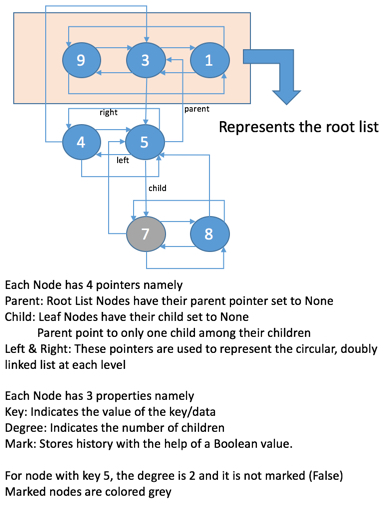
\includegraphics[scale=0.5]{Figures/FibonacciHeap}
